\section{楕円立体解析幾何学}

二重回転面の方程式が得られるところまで展開する。

\begin{figure}[h]
\centering
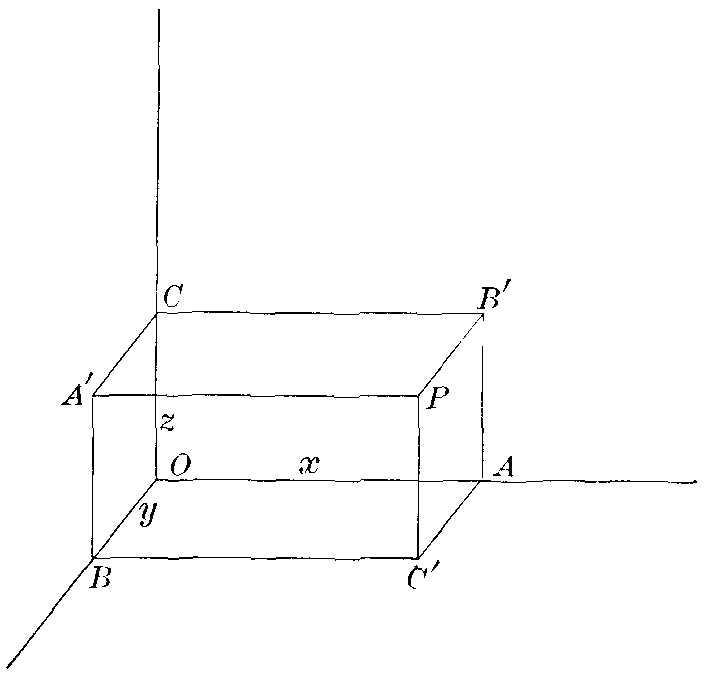
\includegraphics[width=60mm]{fig79.png}
\end{figure}

\begin{description}
\item[1.~座標、直線、平面:]\hfill\break

点を通って軸に垂直な三つの平面を引く。座標 $x$、$y$、$z$ としては、これらの平面が軸上に切り取る切片をとる。

これら三つの平面の交線は、座標平面に垂直である（第I章, II, 16 および 17）。実際、図の面角はすべて直角であるが、$P$ での角と、三つの角 $BA'C$、$CB'A$、$AC'B$ は鈍角である。

$\rho$ を点 $P$ への動径とし、$\alpha$、$\beta$、$\gamma$ をそれが三つの軸となす三つの角とする。すると、
\begin{align*}
  \cos^2\alpha + \cos^2\beta + \cos^2\gamma &= 1,\\
  \cos\alpha &= \frac{\tan x}{\tan\rho},\ \text{など;}\\
  \tan^2x + \tan^2y + \tan^2z &= \tan^2\rho.
\end{align*}

原点で交わる二直線のなす角については、
\begin{equation*}
  \cos\theta = \cos\alpha\,\cos\alpha' + \cos\beta\,\cos\beta'
  + \cos\gamma\,\cos\gamma'.
\end{equation*}

二点 $xyz$ と $x'y'z'$ が原点で張る角は、方程式
\begin{equation*}
  \cos\theta = \frac{\tan x\, \tan x' + \tan y\, \tan y'
    + \tan z\, \tan z'}{\tan\rho\, \tan\rho'}
\end{equation*}
で与えられる。

二点間の距離については、
\begin{equation*}
  \cos\delta = \cos\rho\,\cos\rho' + \sin\rho\,\sin\rho'\,\cos\theta.
\end{equation*}

これから球面の方程式が得られ、$\delta = \frac{\pi}{2}$ のとき平面の方程式が得られる。後者を直交座標で表すと、
\begin{equation*}
  \tan x\, \tan x' + \tan y\, \tan y' + \tan z\, \tan z' + 1 = 0
\end{equation*}
である。

$p$ を原点から平面に下ろした垂線の長さとし、$\alpha$、$\beta$、$\gamma$ をこの垂線が軸となす角とする。するとその極については、
\begin{align*}
  \rho' &= p + \frac{\pi}{2},\\
  \tan x' = \tan\rho'\,\cos\alpha &= -\,\frac{\cos\alpha}{\tan p},\
  \text{など;}
\end{align*}
ゆえに、平面の方程式は次のように書ける。
\begin{equation*}
\cos\alpha\,\tan x + \cos\beta\,\tan y + \cos\gamma\,\tan z
   = \tan p.
\end{equation*}

\item[2.~二重回転面:]\hfill\break

その軸の一つを $z$ 軸にとり、$k$ を曲面からこの軸までの距離とし、$\theta$ を、点 $P$ と $z$ 軸を通る平面が $xz$ 平面となす角とする。$z$ と $\theta$ を緯度と経度と呼ぶことができる。

$OA$ と $CB$ を延長する。それらは、$z$ 軸から距離 $\frac{\pi}{2}$ のところで、曲面の他方の軸上の点 $O'$ で交わり、そこで測度が $z$ に等しい角をなす。

直角三角形 $O'AB$ から、
\begin{align*}
\cos z &= \frac{\tan OA}{\tan O'B}.\\
\intertext{しかるに}
\tan O'A &= \cot x,\\
\intertext{および}
\tan O'B &= \cot CB = \frac{\cot k}{\cos\theta}.\\
\intertext{したがって、}
\cos z &= \frac{\tan k\,\cos\theta}{\tan x},\\
\intertext{すなわち}
\tan x &= \frac{\tan k\,\cos\theta}{\cos z}.\\
\intertext{同様にして、}
\tan y &= \frac{\tan k\,\sin\theta}{\cos z}.\\
\intertext{二乗して加えると、曲面の方程式は}
\tan^2x + \tan^2y &= \tan^2k\sec^2z
\end{align*}
となる。

\begin{figure}[h]
\centering
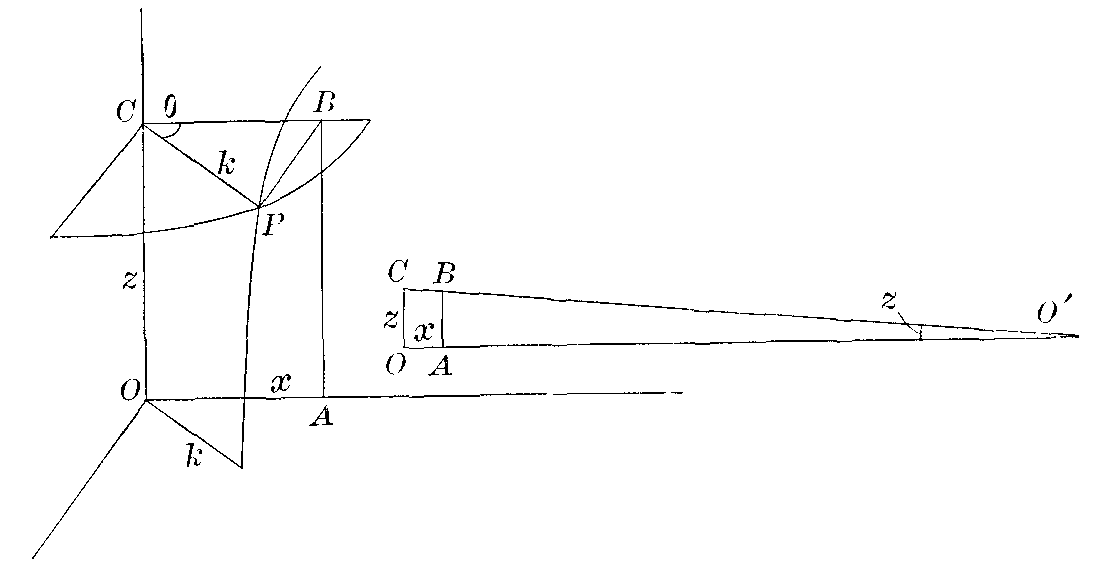
\includegraphics[width=80mm]{fig80.png}
\end{figure}

曲面上の二点を結ぶ弦の長さについては、
\begin{equation*}
\cos\delta = \cos\rho\,\cos\rho'
  (1 + \tan x\,\tan x' + \tan y\,\tan y' + \tan z\,\tan z').
\end{equation*}
さて、
\begin{align*}
\tan^{2}\rho &= \tan^{2}k\,\sec^{2}z + \tan^{2}z; \\
\intertext{したがって、}
\sec^{2}\rho &= \sec^{2}k\,\sec^{2}z,\\
\intertext{すなわち}
\cos\rho &= \cos k\,\cos z. \\
\intertext{すなわち、$z$、$z'$、$\theta$、$\theta'$ で表すと、}
\cos\delta &= \cos^2k\,\cos(z'-z) + \sin^2k\,\cos(\theta'-\theta). \\
\intertext{これから、曲面上の長さの微分要素 $ds$ の表式が得られる。}
\cos ds &= \cos^2k\,\cos dz + \sin^2k\,\cos d\theta, \\
\intertext{あるいは、}
\cos ds &= 1 - \frac{ds^2}{2},\ \text{など,} \text{ であるから} \\
ds^2 &= \cos^2k\, dz^2 + \sin^2k\, d\theta^2.
\end{align*}

$z$ と $\theta$ は、二つの円の系に沿って測った距離に比例する。これらの円は直角に交わり、曲面上の直交座標系を与えるのに用いることができる。これら二つの円の系に沿った実際の長さは $\theta\sin k$ と $z\cos k$ である（第III章の系を見よ）。したがって、
\begin{equation*}
\alpha = \theta\sin k,\quad \beta = z\cos k
\end{equation*}
と書けば、直角に交わるこれら二つの円の系に沿って測った距離を座標とする、曲面上の直交系が得られる。

公式はこのとき
\begin{equation*}
ds^2 = d\alpha^2 + d\beta^2
\end{equation*}
となる。

$\alpha$ と $\beta$ の一次方程式は、この曲面上で、ユークリッド幾何学の平面上の直線のすべての性質をもつ曲線を表す。任意の二点を通って、そのような線がただ一本引ける。二組の座標は、一次方程式の係数を決めるのにちょうど十分だからである。曲面上の二点間の最短距離は、そのような線上で測られる。なぜなら、$\alpha$ と $\beta$ の方程式で表される道に沿った二点間の距離は、$\alpha$ と $\beta$ を直交座標にとったユークリッド平面上の、対応する点と対応する道に沿った距離と同じだからである。したがって、道が $\alpha$ と $\beta$ の一次方程式で表されるときに、それが最短でなければならない。曲面上のそのような線を\emph{測地線}といい、曲面に関するかぎり、直線と呼ぶ。これらの線の一つの上で測った任意の二点間の距離は、公式
\begin{equation*}
d = \sqrt{(\alpha-\alpha')^2 + (\beta-\beta')^2}
\end{equation*}
で表される。

これらの線でつくられる三角形は、ユークリッド幾何学の平面三角形のすべての性質をもつ。角の和は $\pi$ である、などである。実際、この曲面と楕円空間との関係は、限界面と双曲空間との関係と同じである。

直線の方程式の標準形は、
\begin{equation*}
\alpha\cos\omega + \beta\sin\omega = p
\end{equation*}
である。

曲面の直線の母線は、$z$ 軸の極線である軸のまわりに描いたすべての円と、一定の角 $\pm k$ をなす。したがってこれらの母線は曲面上の「直線」であり、その方程式は次の形になる。
\begin{equation*}
\alpha\cos k \pm \beta\sin k = p.
\end{equation*}
\end{description}
